\section{Entraînement du modèle}%
\label{sec.results.training}

Tous les tests présentés dans le reste de ce chapitre ont été effectués sur un ordinateur portable 
équipé d'un processeur \verb|Intel Core i9-8950HK| et d'une carte graphique \verb|NVIDIA GeForce GTX 1050 Ti|.
Cette machine dispose de 32 Go de mémoire vive et de 4 Go de mémoire vidéo.
Le système d'exploitation est \verb|Ubuntu 20.04 LTS|, 
la version de Python utilisée est \verb|3.10.6|
et celle de CUDA est \verb|11.6.124|.

L'entraînement du modèle a été effectué en suivant la procédure illustrée par la figure~\ref{fig.results.training}.
\begin{figure}[hbt]
    \begin{center}
        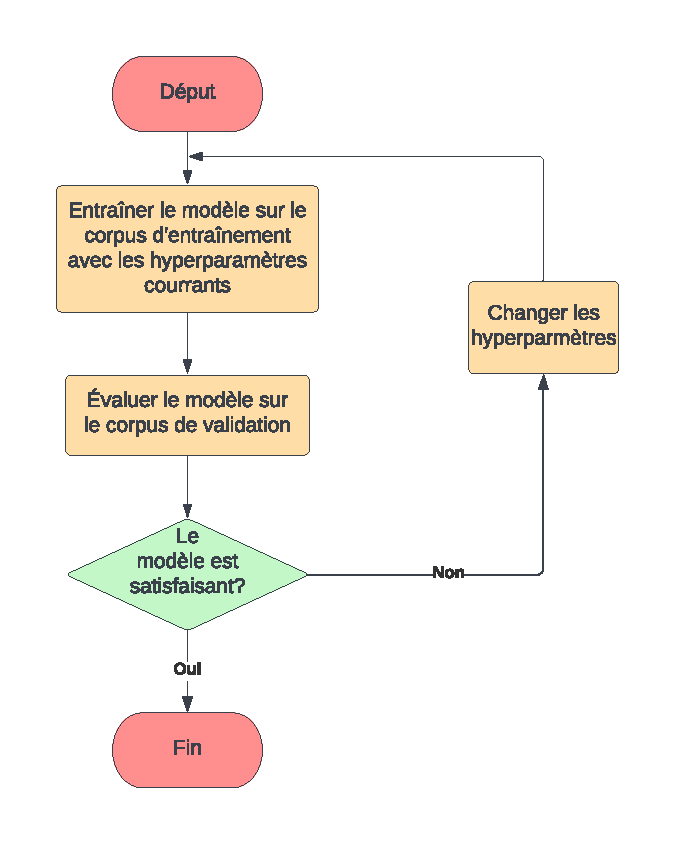
\includegraphics[width=6cm]{assets/pdf/Training.pdf}
    \end{center}
    \caption{Organigramme de la phase d'entraînement}%
    \label{fig.results.training}
\end{figure}
Le modèle est d'abord entraîné avec un choix d'hyperparamètres plus ou moins arbitraire
pour vérifier que l'entraînement se déroule correctement.
Ensuite, une recherche d'hyperparamètres est effectuée pour trouver les meilleurs hyperparamètres.
Cette recherche est effectuée uniquement si l'entraînement initial n'a pas donné des résultats satisfaisants.


\subsection{Choix des hyperparamètres}%
\label{sub.results.training.hyperparameters}

Pour notre premier test, nous avons entraîné le modèle pour 8 époques (cela a pris 58~min~25~s).
Les hyperparamètres ont été choisis comme suit :
\begin{itemize}
    \item Dimension de plongement : 64
    \item Dimension de la couche cachée : 64
    \item Taux d'apprentissage : \(3 \cdot 10^{-4}\)
    \item Dropout : 0.1
    \item Nombre de couches de l'encodeur/décodeur : 3
    \item Nombre de têtes d'attention : 4
    \item Norme maximale des plongements : 1
    \item Taille de lot : 256
    \item Norme maximale du gradient : 1
    \item Coefficient de régularisation \(L_2\) : \(10^{-4}\)
    \item Nombre de processus pour le chargement des données : 4
\end{itemize}


\subsection{Entraînement initial}%
\label{sub.results.training.initial}

L'objectif de ce test est de vérifier que le modèle fonctionne correctement.
Cela inclut la vérification du bon déroulement du chargeur de données,
des passes \foreignlanguage{english}{forward} et \foreignlanguage{english}{backward}
et l'absence de sur-apprentissage.
La probabilité de ce dernier point n'est pas négligeable dans notre cas,
car le modèle est grand en comparaison avec la complexité de la procédure de génération des données.

Pour chaque époque, nous avons calculé la moyenne de la fonction de perte, de l'exactitude et du score \gls{bleu} 
sur le corpus de validation et sur le corpus d'entraînement.
Les résultats de ce test sont présentés dans la Figure~\ref{fig.results.over}.
\begin{figure}[hbt]
    \begin{subfigure}{.5\textwidth}
        \caption{Exactitude}
        \begin{center}
            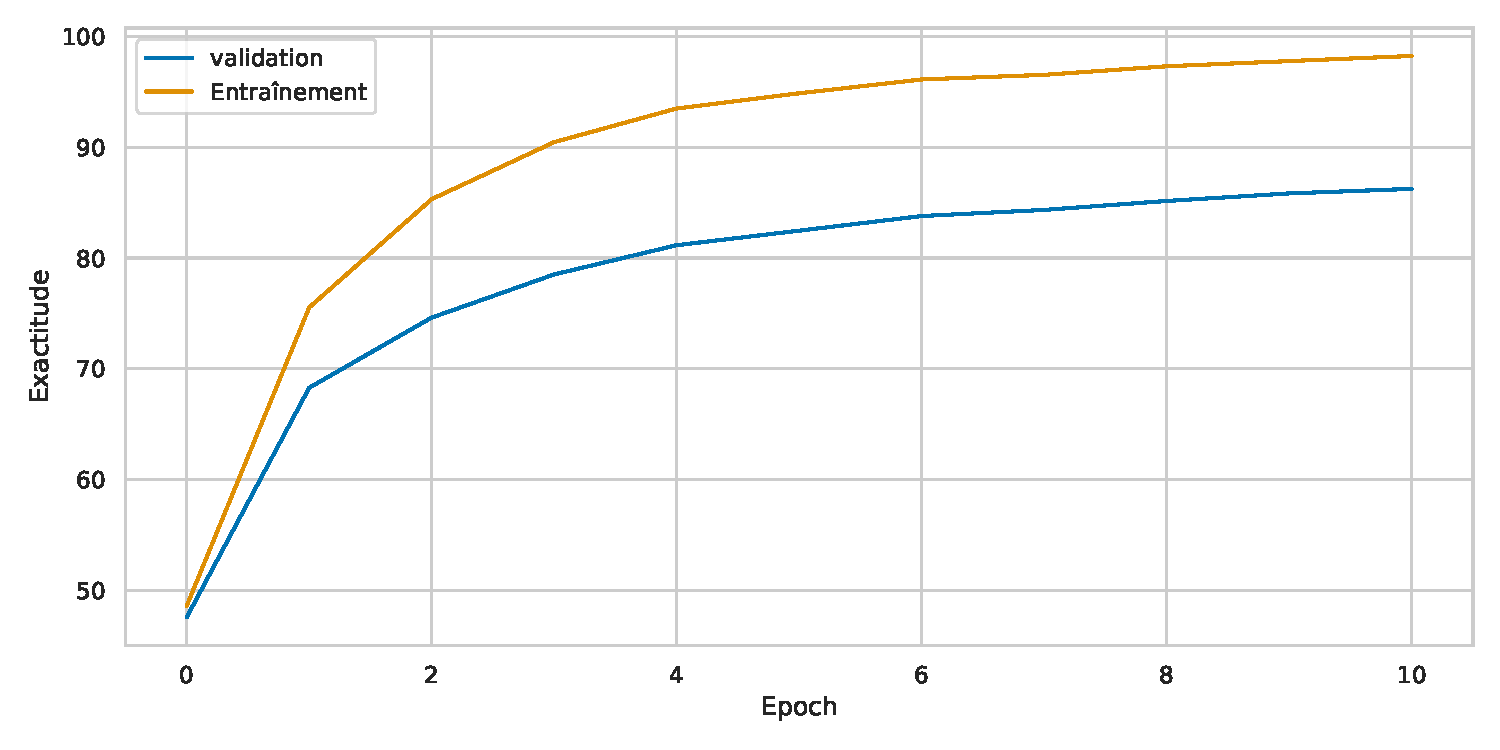
\includegraphics[width=\textwidth]{assets/python/over-accuracy.pdf}
        \end{center}
        \label{fig.results.over.accuracy}
    \end{subfigure}
    \begin{subfigure}{.5\textwidth}
        \caption{\glsfmtshort{bleu}}
        \begin{center}
            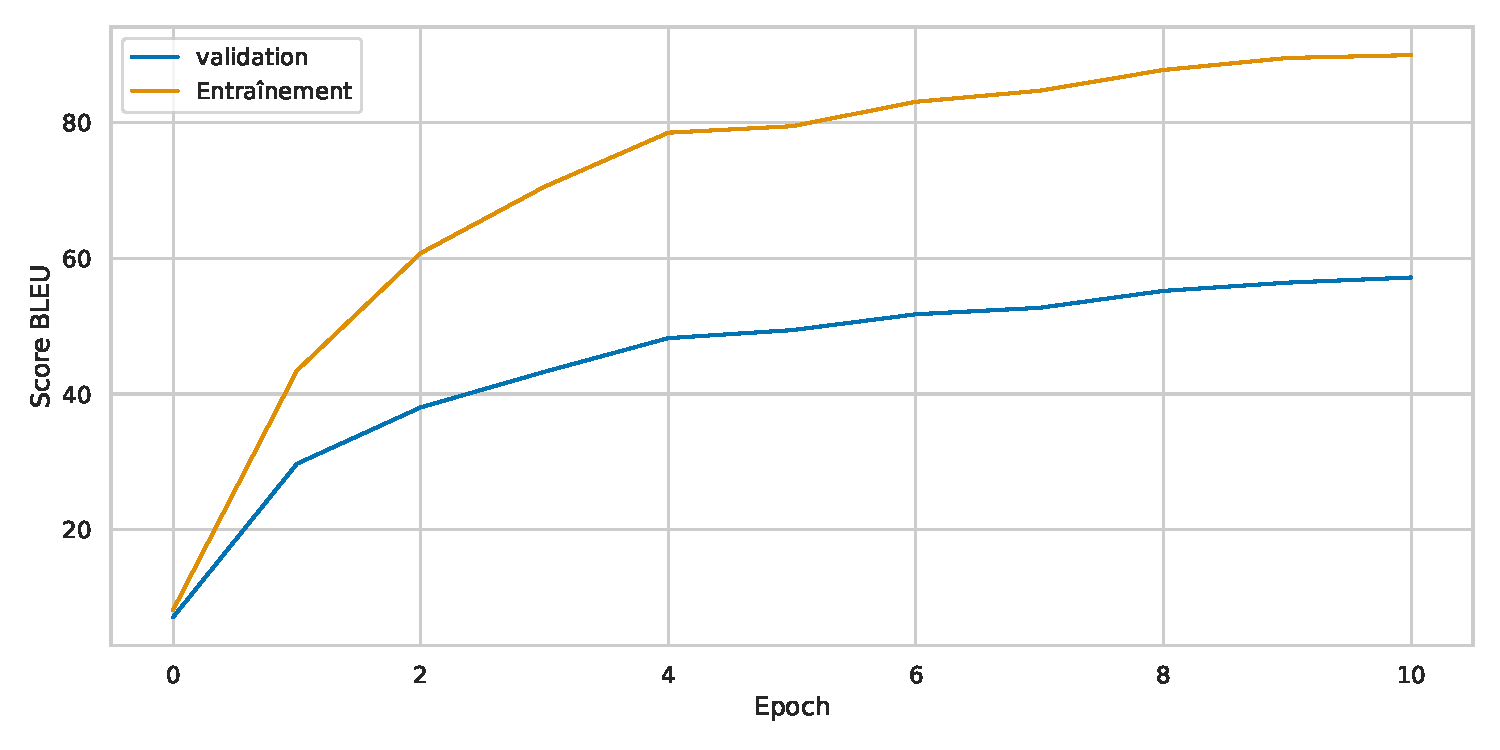
\includegraphics[width=\textwidth]{assets/python/over-bleu.pdf}
        \end{center}
        \label{fig.results.over.bleu}
    \end{subfigure}
    \begin{subfigure}{.5\textwidth}
        \begin{center}
            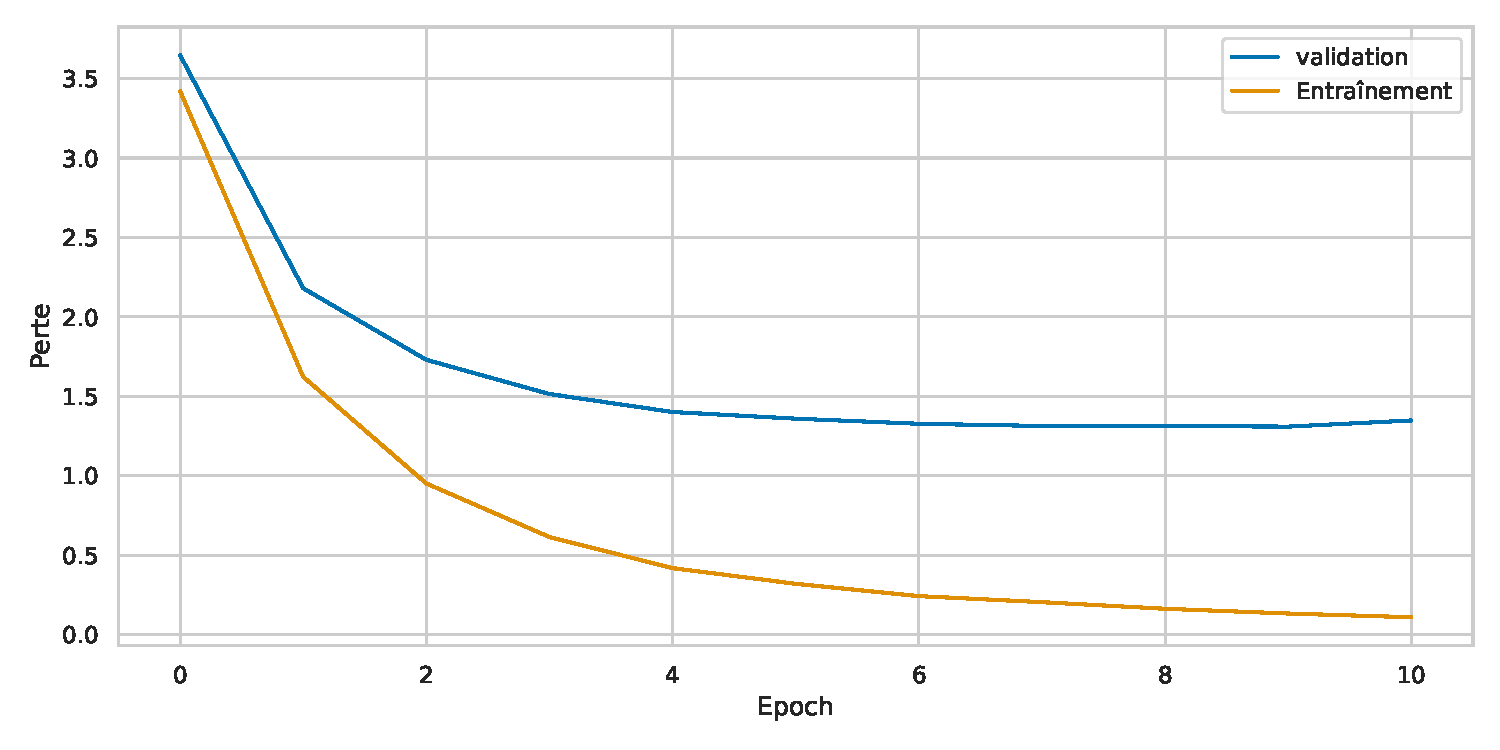
\includegraphics[width=\textwidth]{assets/python/over-loss.pdf}
        \end{center}
        \caption{Perte}
        \label{fig.results.over.loss}
    \end{subfigure}
    \caption{Évolution des métriques au cours de l'entraînement.}
    \label{fig.results.over}
\end{figure}
Ces résultats montrent que l'entraînement ne présente pas d'anomalies.
Les 11 premières époques se déroulent sans erreurs et les métriques évoluent comme prévu.
Cependant, la Figure~\ref{fig.results.over.loss} montre des signes clairs de sur-apprentissage.
L'écart entre les courbes d'entraînement et de validation est très important.

Comme évoqué précédemment, ce résultat n'est pas surprenant.
En effet, le modèle peut apprendre les règles de substitution utilisées pour générer les erreurs
plutôt que la correspondance entre la phrase d'origine et la phrase erronée.
Il est donc nécessaire de trouver une façon de forcer le modèle à apprendre la correspondance entre les phrases.

\subsection{Entrainement avec les erreurs masquées}%
\label{sub.results.masking}

Pour remédier au problème de sur-apprentissage rencontré lors de l'entraînement initial,
nous avons bruité les données d'entraînement.
Pour empêcher le modèle d'apprendre les règles de substitution,
nous avons masqué les erreurs en les remplaçant par le token \verb|[UNK]|.
Cette technique est inspirée du \gls{mlm} de \gls{bert}~\cite{Devlin_Chang_Lee_Toutanova_2019}
et de l'auto-encodage de \gls{bart}~\cite{Lewis_Liu_Goyal_Ghazvininejad_Mohamed_Levy_Stoyanov_Zettlemoyer_2019}.

\begin{figure}[hbt]
    \begin{subfigure}{.5\textwidth}
        \caption{Exactitude}
        \begin{center}
            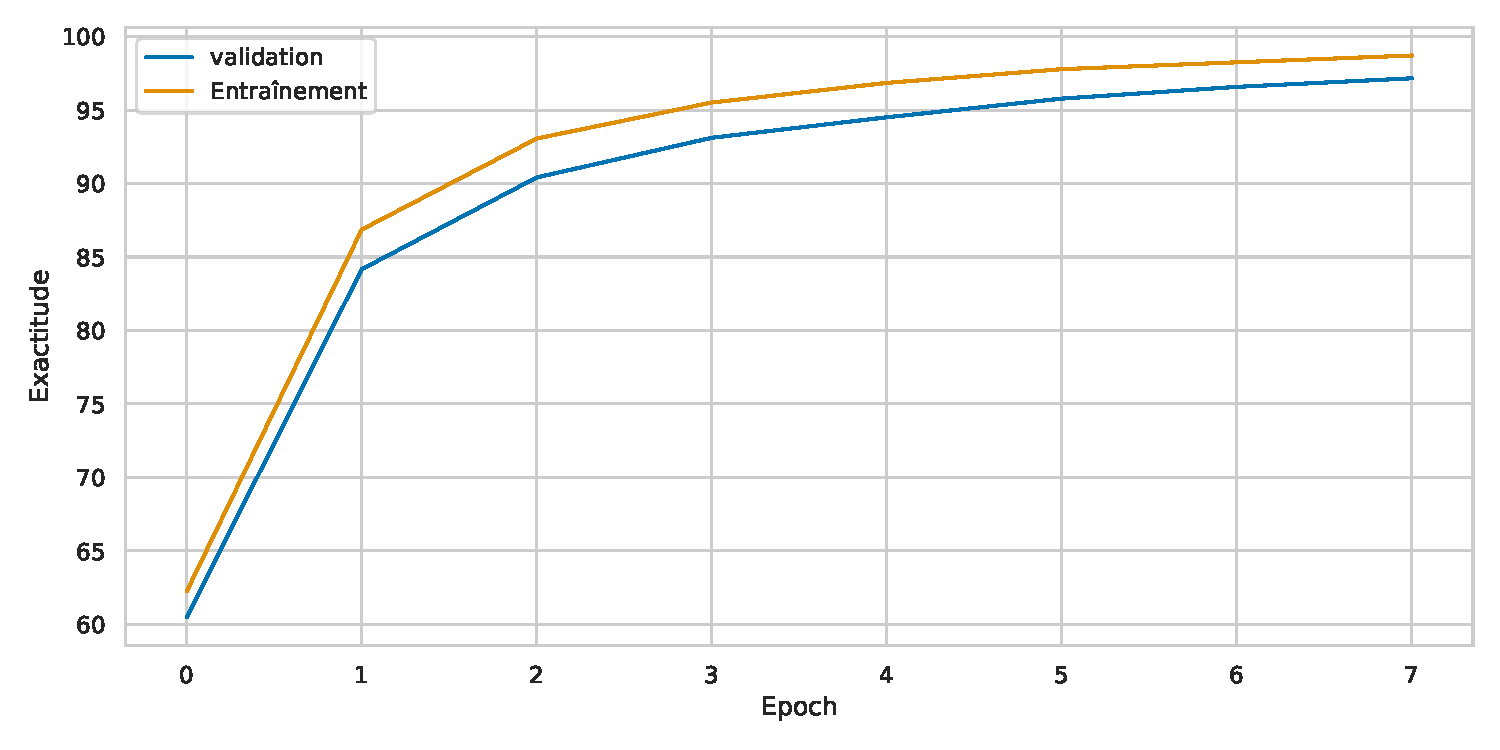
\includegraphics[width=\textwidth]{assets/python/accuracy.pdf}
        \end{center}
        \label{fig.results.training.accuracy}
    \end{subfigure}
    \begin{subfigure}{.5\textwidth}
        \caption{\glsfmtshort{bleu}}
        \begin{center}
            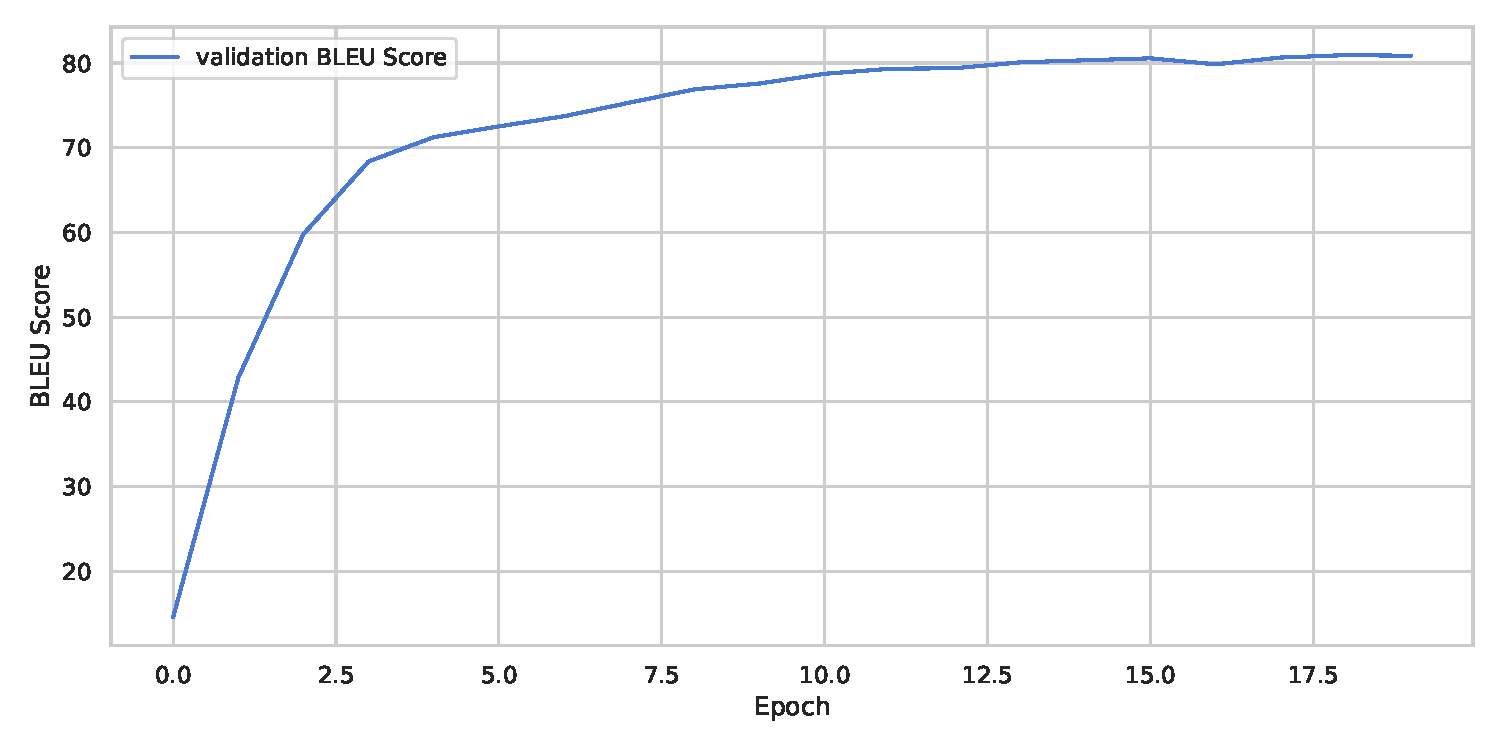
\includegraphics[width=\textwidth]{assets/python/bleu.pdf}
        \end{center}
        \label{fig.results.training.bleu}
    \end{subfigure}
    \begin{subfigure}{.5\textwidth}
        \begin{center}
            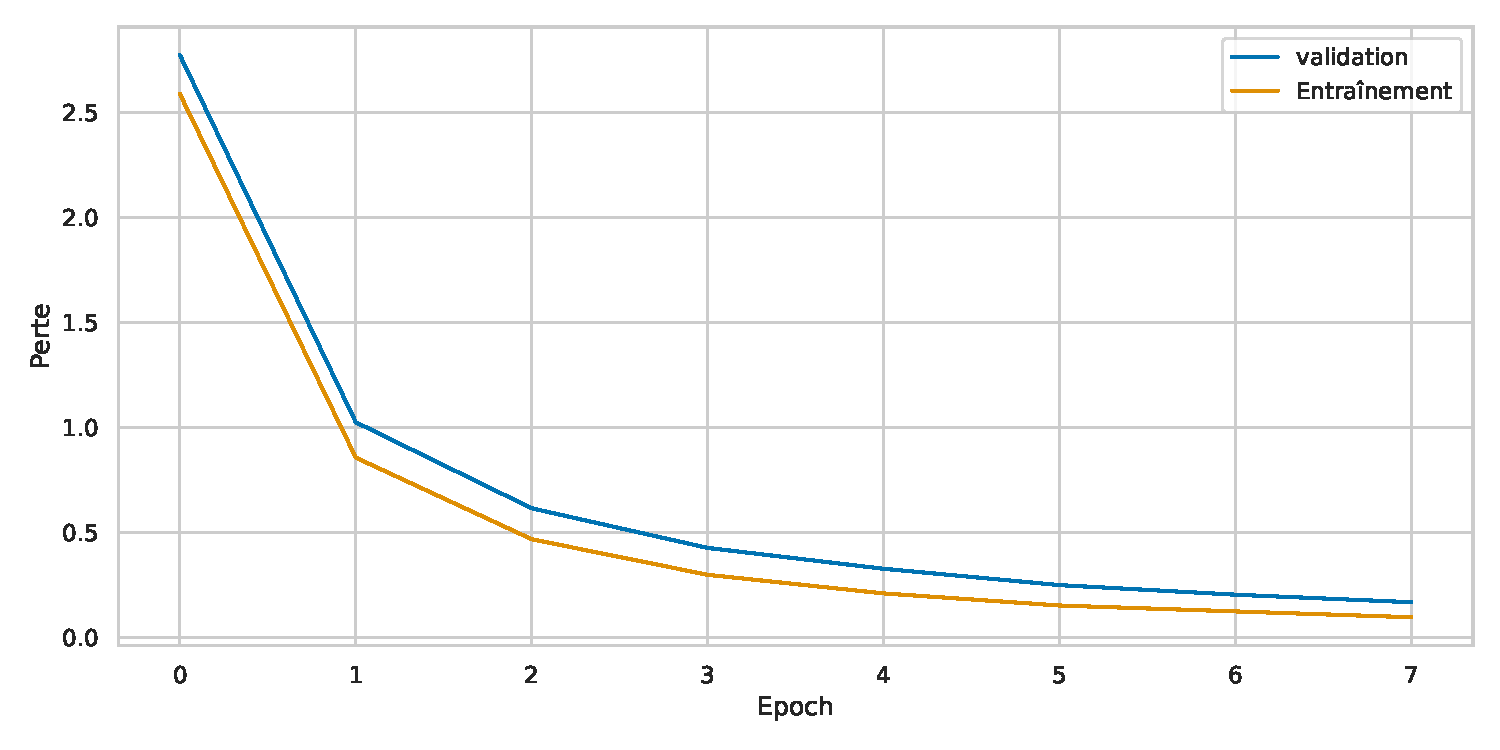
\includegraphics[width=\textwidth]{assets/python/loss.pdf}
        \end{center}
        \caption{Perte}
        \label{fig.results.training.loss}
    \end{subfigure}
    \caption{Évolution des métriques au cours de l'entraînement.}
    \label{fig.results.training}
\end{figure}
Les résultats sont présentés dans la Figure~\ref{fig.results.training}.
Au bout de 8 époques, la perte sur le corpus d'entraînement est de \(0.09\).
L'exactitude est de \(98.71\%\) et le score \gls{bleu} est de \(81.41\%\).
Les résultats sur le corpus de validation sont comparables.
Les mêmes métriques valent respectivement \(0.16\), \(97.16\%\) et \(77.38\%\).

Les courbes de la Figure~\ref{fig.results.training} montrent 
une forte correspondance entre les courbes d'entraînement et de validation.
Cela suggère que le modèle ne sur-apprenne plus les erreurs.
On note également que les pentes des trois courbes ne sont pas négligeables.
Il est donc probable que le modèle puisse encore s'améliorer en augmentant le nombre d'époques.